\section{Potenciální versus aktuální nekonečno}\label{sec:pot_vs_akt_nekonecno}

Co je vlastně nekonečno? Čtenáři toho může připadat jako absurdní dotaz,~ale tento zdánlivě jasný pojem způsoboval ve své době potíže.\par
Fakt, že přirozených čísel je nekonečně mnoho byl znám již ve starověku.
\begin{equation*}
1,2,3,\dots
\end{equation*}
I žáci na základních školách jsou si této skutečnosti vědomi~a pravděpodobně se nad tím nikdo z nich nepozastaví. Jak~ale toto můžeme chápat? Existují dva základní způsoby.\par
Pokud začneme postupně vypisovat všechna přirozená čísla, jistě je nikdy nevypíšeme všechna, protože bez ohledu na to, jakou si zvolíme mez, vždy ji nakonec přesáhneme. Takovémuto nekonečnému \textbf{procesu} pak říkáme \emph{potenciální nekonečno}.\par
Druhou možností~ale je, že se na množinu přirozených čísel budeme dívat již jako na "hotovou". To znamená, že nebudeme řešit, jak všechna přirozená čísla vypíšeme,~ale budeme na tuto množinu nahlížet již jako na \textbf{celek}, tedy nekonečno budeme chápat v uzavřené formě. V takovém případě mluvíme o tzv. \emph{aktuálním nekonečnu}.
\medskip

Starým Řekům se~však jak z důvodů matematických, tak filozofických, zdálo, že lidskému myšlení je přístupné pouze nekonečno \textbf{potenciální}. O tom se lze přesvědčit už ze samotných \emph{Eukleidových axiómů}. K axiomatice čtenář bude mít možnost blíže nahlédnout v kapitole \ref{chap:axiomy_tm}. \name{Eukleidés} právě z důvodu nemyslitelnosti aktuálního nekonečna mluvil o \emph{přímce} jako o úsečce, kterou může libovolně prodlužovat, nikoliv, že je "nekonečná"~nebo "nekonečně dlouhá", jak říkáme dnes.

\subsection{Galileova úvaha o velikosti}
\label{subsec:galileo}

S problémem nekonečna se~však pojily~i další problémy. Při zrodu samotné teorie množin v 70. letech 19. století se~totiž nabízela otázka, zdali \emph{má vůbec smysl porovnávat nekonečné množiny}. Nad tím se pozastavil už jeden z géniů 16.~a 17. století \name{Galileo Galilei} (1564--1642). Ten si vypsal dvě posloupnosti čísel:
\begin{align*}
1,\ 2,\ 3,\dots,\ n,\dots \quad \text{a} \quad 1,\ 4,\ 9,\dots,\ n^2,\dots ,
\end{align*}
tzn. přirozená čísla~a jejich druhé mocniny. Avšak při pohledu na tyto dvě posloupnosti si Galileo uvědomil, že každý prvek množiny přirozených čísel lze "spárovat" s jeho druhou mocninou (v dnešní terminologii bychom řekli, že existuje \emph{bijekce}; na tu se blíže podíváme v sekci \ref{sec:zobrazeni}).

\begin{figure}[H]
	\centering
	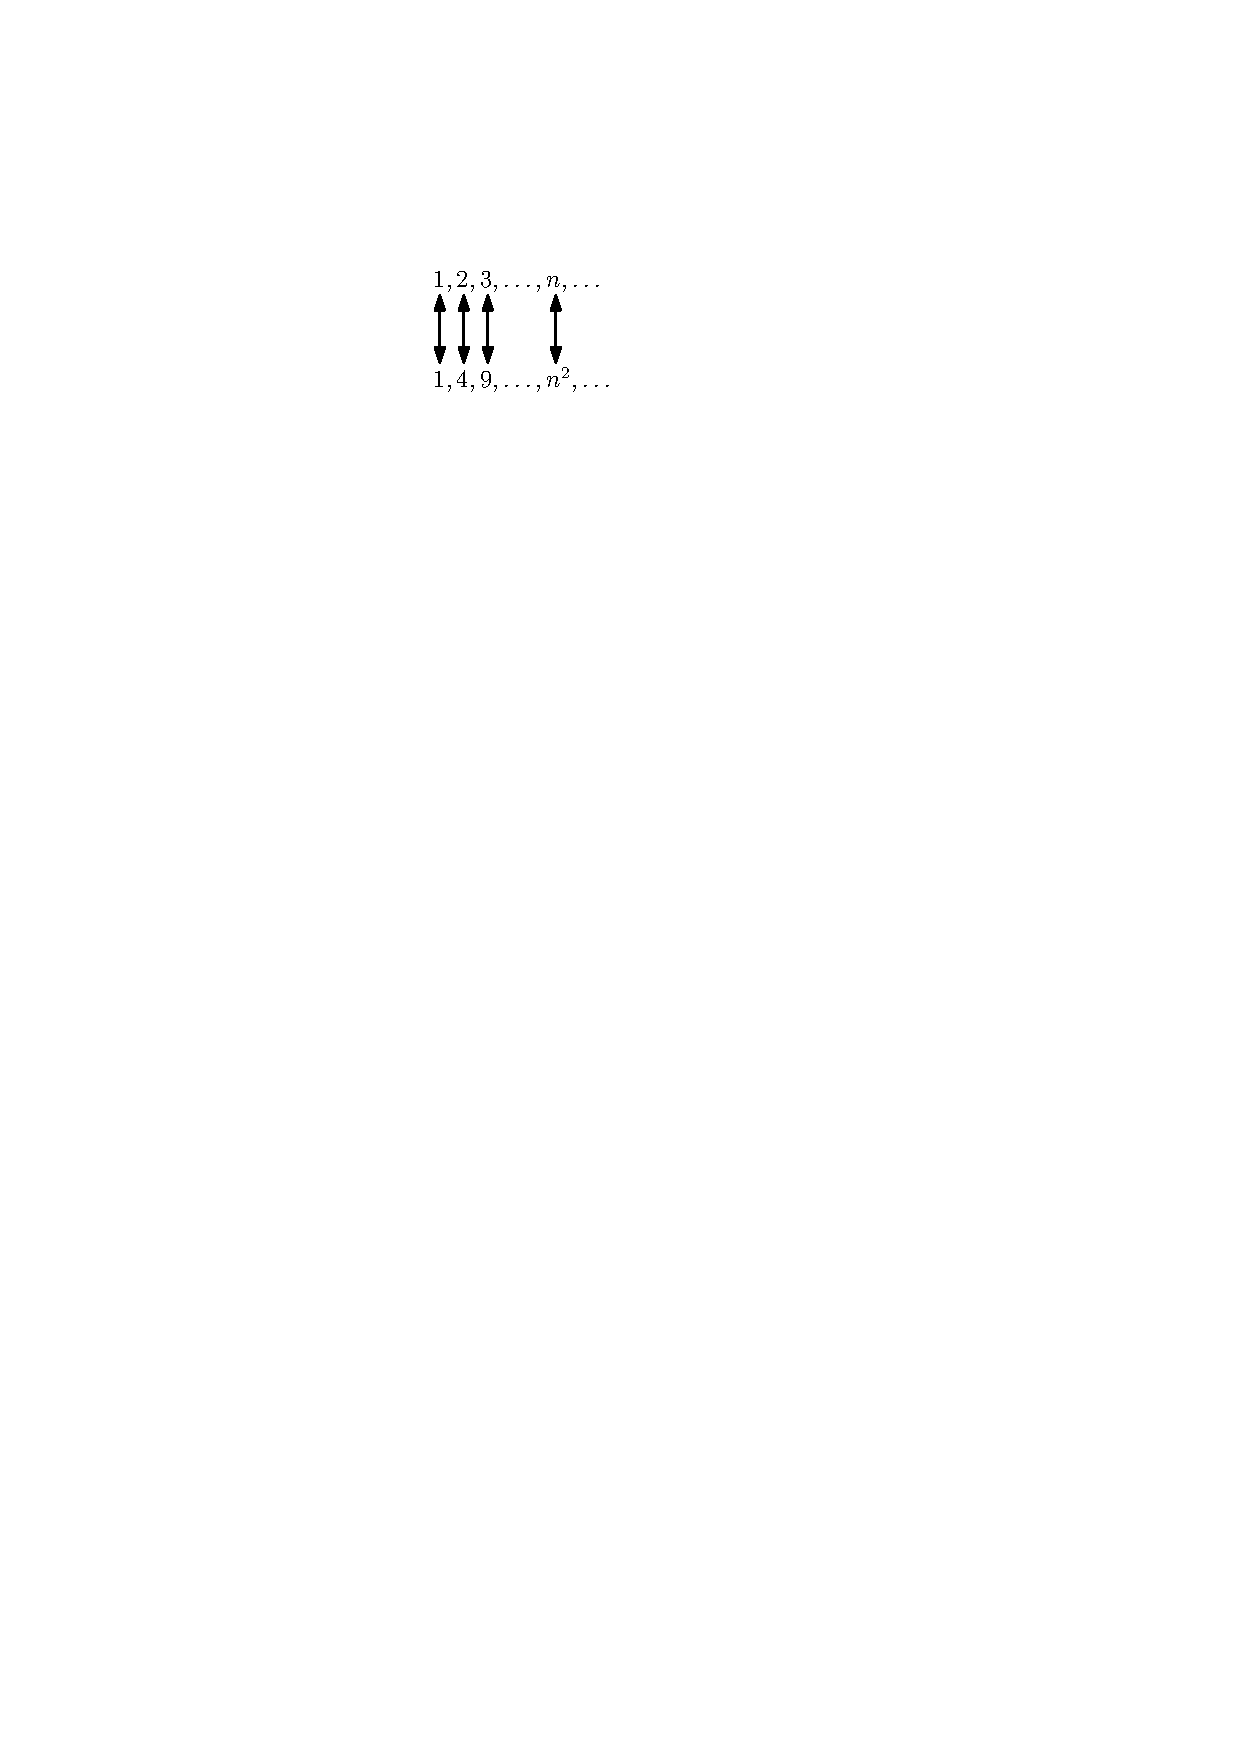
\includegraphics[scale=\normalipe]{ch01_parovani.pdf}
\end{figure}

To by~však znamenalo, že přirozených čísel~a jejich druhých mocnin je \textbf{stejně mnoho}! Avšak jeden z Eukleidových logických axiomů říká, že \emph{celek je větší část}. Proto se tehdy Galileovi zdál tento závěr jako naprostý nesmysl~a tak usoudil, že porovnávat nekonečné množiny podle velikosti zkrátka nemá žádný smysl. Jinak řečeno, tvrdil, že \textbf{aktuální nekonečno} je sporné~a tedy nemůže existovat. \cite{Fuchs2003}% s. 103--105

\subsection{Grandiho řada}

Dalším typickým problémem týkajícího se nekonečna je tzv. \emph{Grandiho řada}. Čtenář se nejspíše již s řadami setkal na střední škole, specificky s řadou aritmetickou~a geometrickou. Řadou v matematice rozumíme zápis
\begin{align*}
a_1+a_2+a_3+\cdots+a_n,
\end{align*}
kde pro všechna přirozená $i$ je $a_i$ člen nějaké posloupnosti. U řad nás celkem pochopitelně zajímal jejich součet. To nebyl většinou problém, neboť jsme se převážně zajímali o řady konečné (a speciálně pro aritmetickou~a geometrickou posloupnost jsme měli~i elegantní vzorce),~ale uvážíme-li řady nekonečné, mohou nastat potíže.\par
Co se vůbec rozumí pod pojmem "součet nekonečné řady"? Jako příklad si vezměme řadu
\begin{equation*}
	\dfrac{1}{2}+\dfrac{1}{4}+\dfrac{1}{8}+\dfrac{1}{16}+\cdots,
\end{equation*}
tedy sčítáme členy posloupnosti $\set{1/2^n}_{n=1}^{\infty}$. Podívejme se, jak se situace bude vyvíjet, když budeme členy postupně přičítat:
\begin{align*}
	\dfrac{1}{2}&=0{,}5\\
	\dfrac{1}{2}+\dfrac{1}{4}&=0{,}75\\
	\dfrac{1}{2}+\dfrac{1}{4}+\dfrac{1}{8}&=0{,}875\\
	\dfrac{1}{2}+\dfrac{1}{4}+\dfrac{1}{8}+\dfrac{1}{16}&=0{,}9375.\\
\end{align*}
Těmto součtům se říká tzv. \emph{částečné součty}. Po součtu prvních dvaceti členů bude výsledek následující:
\begin{equation*}
	\dfrac{1}{2}+\dfrac{1}{4}+\dfrac{1}{8}+\dfrac{1}{16}+\cdots+\dfrac{1}{2^{20}}=0{,}999999046.
\end{equation*}
Jak je vidět, částečné součty se postupně "blíží" nejspíše číslu 1. Dávalo by tedy smysl prohlásit číslo 1 za výsledek této nekonečné řady, tj.
\begin{equation*}
	\dfrac{1}{2}+\dfrac{1}{4}+\dfrac{1}{8}+\dfrac{1}{16}+\cdots=1.
\end{equation*}
Tímto způsobem obecně vnímáme součet nekonečné řady: \textbf{hodnota, ke které se blíží částečné součty}. (Formální definici součtu nekonečné řady si zde odpustíme.)
\medskip

Problému s nekonečnými řadami si všiml italský matematik \name{Gildo Grandi} (1671--1742). Uvažme následující rovnost:
\begin{align*}
0=0+0+0+\cdots .
\end{align*}
To nejspíše nevypadá nikterak zajímavě. Přeci jen nekonečným sčítáním nul celkem přirozeně nemohu dostat jiný výsledek než opět nulu. Nulu si~však můžeme vyjádřit jako $1-1$. Aplikací na rovnost výše dostaneme
\begin{align}
\label{eq:grandiho_rada_uzavorkovana}
0=(1-1)+(1-1)+(1-1)+\cdots .
\end{align}
Podle asociativního zákona pro sčítání můžeme změnit uzávorkování. Změníme jej proto takto
\begin{align*}
0=1+(-1+1)+(-1+1)+(-1+1)+\cdots
\end{align*}
a nakonec z každé závorky vytkneme znaménko "$-$"
\begin{align*}
0=1-(1-1)-(1-1)-(1-1)-\cdots .
\end{align*}
Tedy dostáváme, že
\begin{align*}
0&=(1-1)+(1-1)+(1-1)+\cdots \\ &= 1+(-1+1)+(-1+1)+(-1+1)+\cdots \\ &= 1-(1-1)-(1-1)-(1-1)-\cdots \\ &= 1-0-0-0-\cdots = 1 .
\end{align*}
Aplikací jednoduchých aritmetických pravidel jsme dospěli k závěru, že $0=1$. To je samozřejmě nesmysl,~ale kde je tedy chyba? (Zde poprosím čtenáře, aby se zkusil zamyslet.)\par
\emph{Grandiho řadou} nazýváme zápis
\begin{align*}
1-1+1-1+1-1+\cdots ,
\end{align*}
kterou jsme obdrželi u rovnosti \eqref{eq:grandiho_rada_uzavorkovana} (až na uzávorkování). Není těžké si všimnout, že postupným sčítáním jednotlivých členů se budou částečné součty opakovat
\begin{align*}
1&=1 ,\\
0&=1-1 ,\\
1&=1-1+1 ,\\
0&=1-1+1-1 ,\\
&\vdots
\end{align*}
Zkusme k této řadě přistoupit ještě jedním způsobem. Uvažujme, že řada má součet, který si označíme $S$. Pak
\begin{align*}
S=1-1+1-1+\cdots .
\end{align*}
Opět využitím asociativního zákona~a vytknutím znaménka "$-$" si upravíme řadu na pravé straně takto:
\begin{align*}
S=1-(1-1+1-1+\cdots ) .
\end{align*}
Čtenář si~však již možná všiml, že výraz v závorce na pravé straně je opět námi vyšetřovaná řada se součtem $S$, tedy z toho vyplývá
\begin{align*}
S&=1-S\\
S&=\frac{1}{2} .
\end{align*}
Toto je~však také zarážející výsledek, neboť jak jsme se sami přesvědčili, tak částečné součty pouze oscilují mezi 0~a 1.\par
Všimněme si, že rovnosti uvedené výše jsme obdrželi pouhou aplikací základních početních pravidel; přesto jsou~však sporné. Tyto výsledky později vedly k novým poznatkům v aritmetice,~a to sice faktu, že asociativita~a komutativita definitivně platí pouze u konečných součtů.

\subsection{Nekonečno v matematické analýze}

Velká část matematické analýzy je založená na úvahách s \emph{nekonečně malými veličinami}; často se mluví o tzv. \emph{infinitezimálním počtu}. Čtenář se s těmito pojmy již možná setkal, ačkoliv nemusí mít nutně představu o jeho přesném významu. Asi nejznámějším příkladem je integrální počet, specificky výpočet "plochy pod křivkou".
\begin{figure}[H]
	\centering
	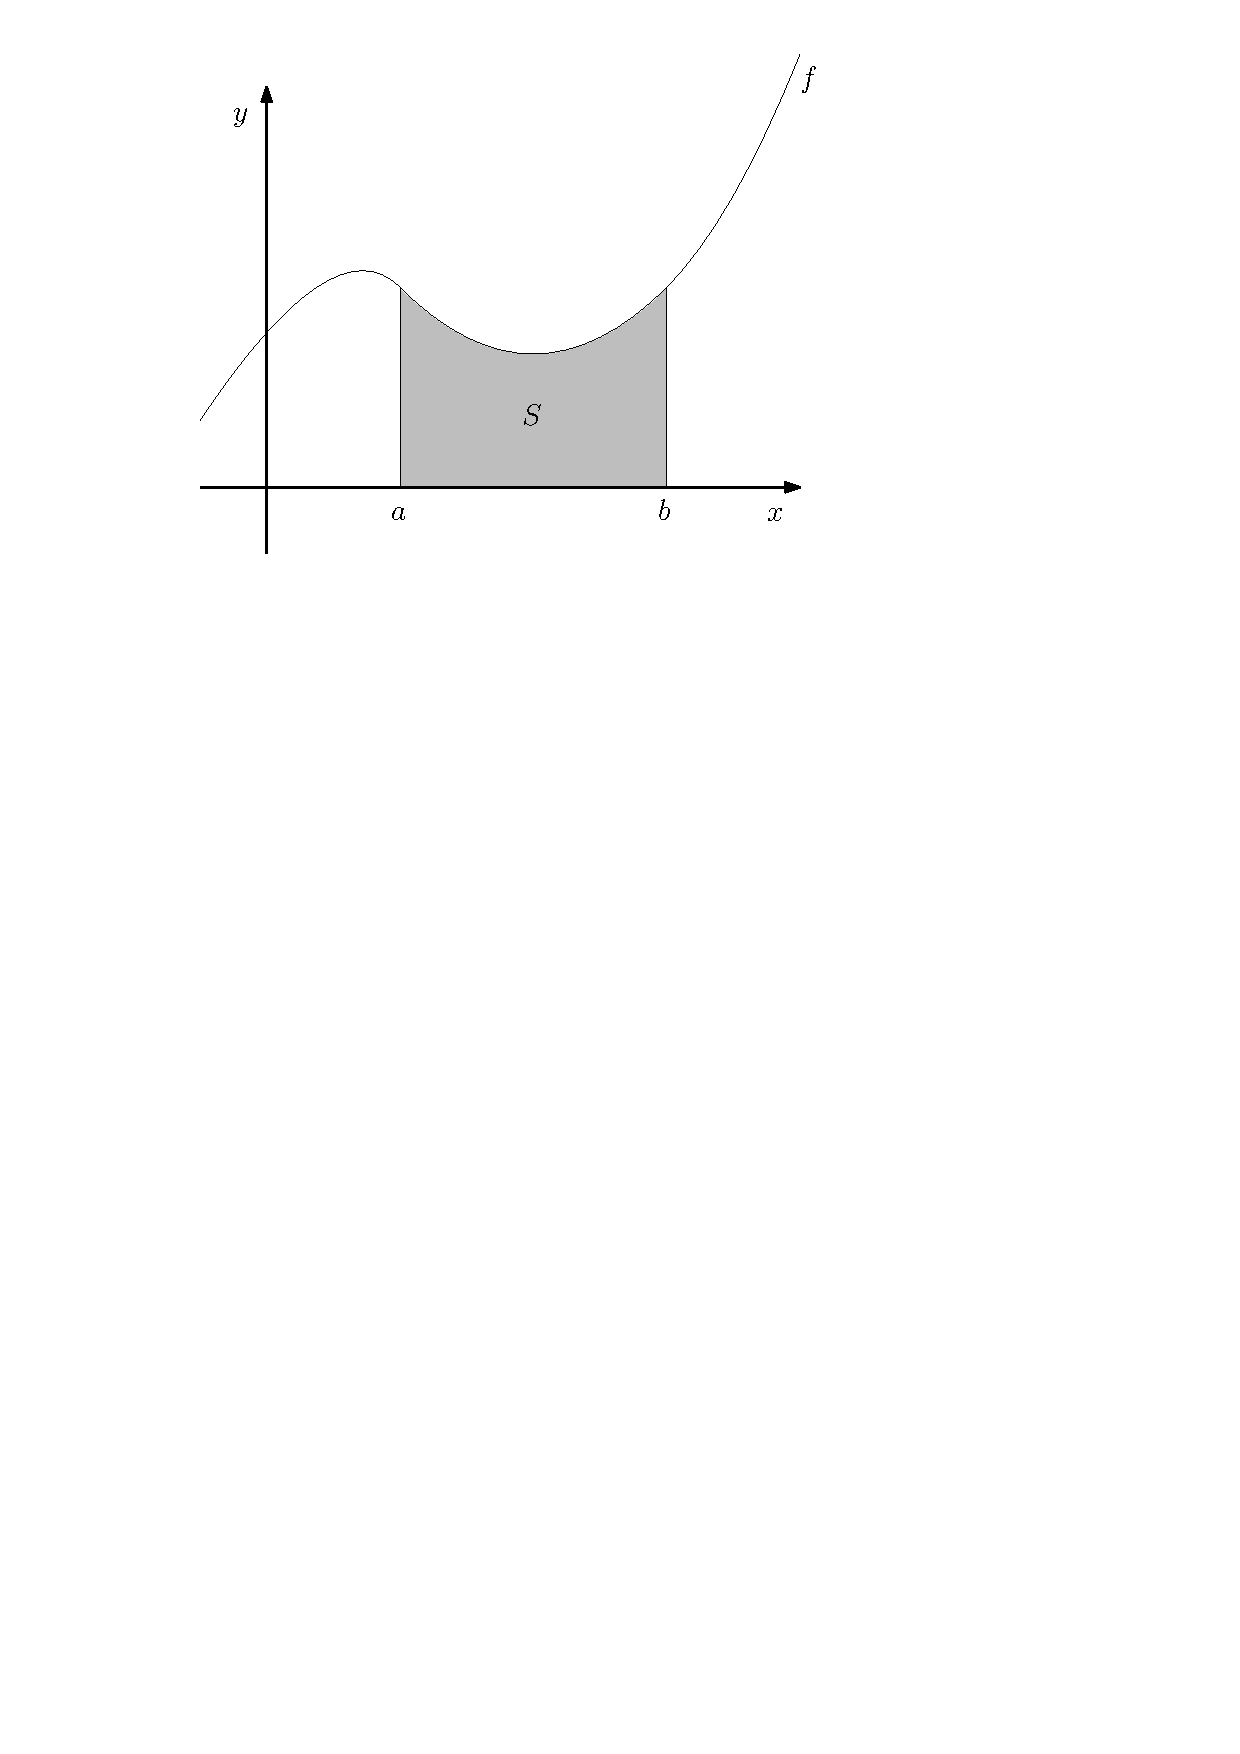
\includegraphics[scale=\normalipe]{ch01_urcity_integral_ukazka.pdf}
	\caption{Příklad určitého integrálu funkce $f$ na uzavřeném intervalu $\langle a,b \rangle$.}
	\label{fig:urcity_integral_ukazka}
\end{figure}

Obrázek \ref{fig:urcity_integral_ukazka}~a obrázky jemu podobné se často uvádí ve spojitosti s tzv. \emph{určitým integrálem}. Zde bychom mohli psát
\begin{align*}
S=\int_{a}^{b}{f(x)\,\dx{}}.
\end{align*}
Pro upřesnění, pokud platí, že funkce $f$ je na intervalu $\langle a,b \rangle$ kladná, pak integrál $\int_a^b{f(x)\,\dx{}}$ je obsah plochy pod grafem funkce $f$ na intervalu $\langle a,b \rangle$. Výpočet obsahu takové složitě vypadající plochy, jako na obrázku \ref{fig:urcity_integral_ukazka}, se může zdát bez znalosti integrálního počtu takřka nemožným úkolem. Pokusme se~ale na danou problematiku podívat právě optikou infinitezimálního počtu. (Znalý čtenář snad promine, že se zatím zdržím formalismů~a pouze jednoduše naznačím myšlenku.)\par
Pro začátek zkusíme plochu pouze aproximovat. K tomu využijeme tvar, jehož obsah jsme schopni triviálně vypočítat -- obdélníka. Pro začátek zkusíme plochu aproximovat pomocí 4 obdélníků (viz obrázek \ref{fig:urcity_integral_aproximace1}).
\begin{figure}[H]
	\centering
	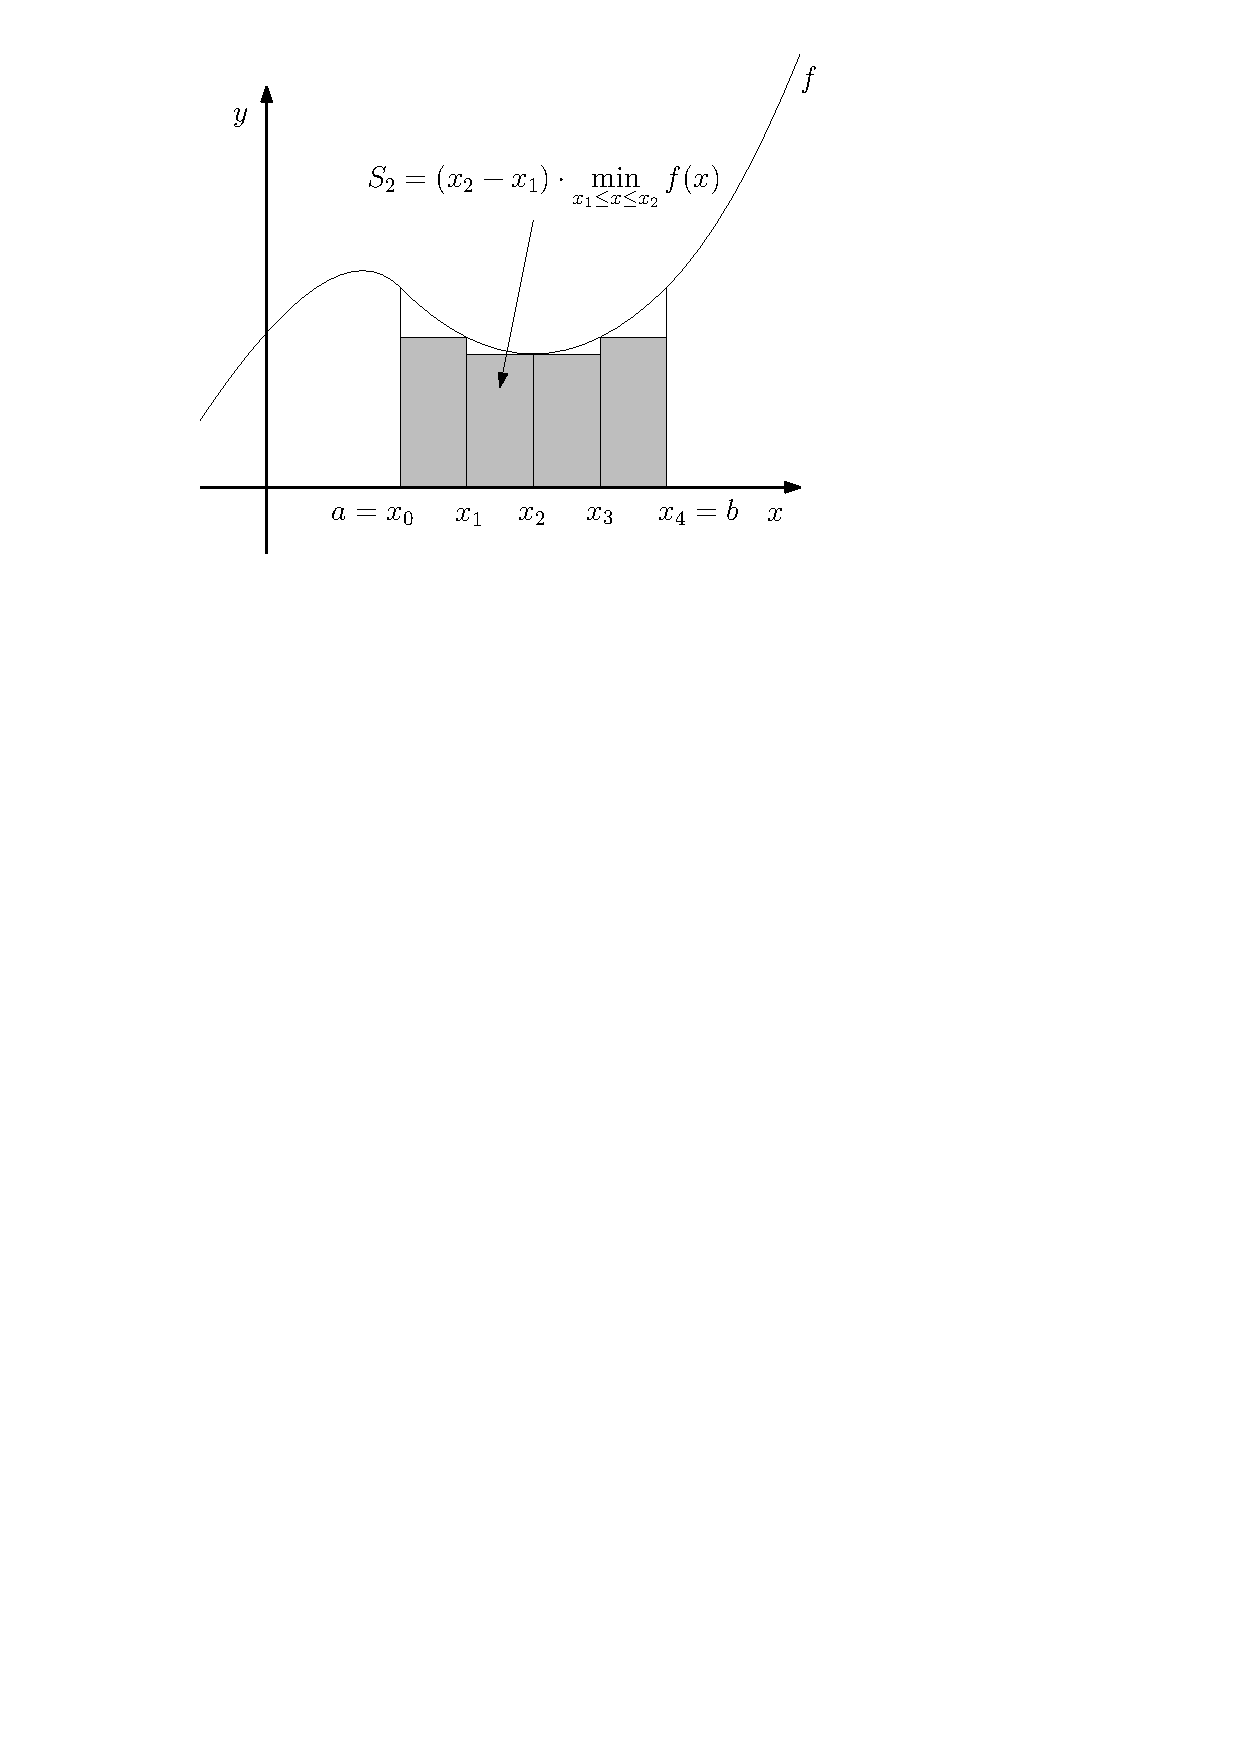
\includegraphics[scale=\normalipe]{ch01_urcity_integral_aproximace1.pdf}
	\caption{Aproximace plochy pod grafem funkce $f$ na intervalu $\langle a,b \rangle$ pomocí 4 obdélníků.}
	\label{fig:urcity_integral_aproximace1}
\end{figure}
Všechny 4 obdélníky jsme zvolili tak, aby měly stejnou šířku~a jejich výška odpovídala minimální hodnotě v daném dílčím intervalu. Obecně obsah $i$-tého obdélníku $S_i$ bychom zapsali jako
\begin{align*}
S_i= (x_i-x_{i-1}) \cdot \min\limits_{x_{i-1} \leq x \leq x_i}{f(x)},
\end{align*}
kde $\min_{x_{i-1} \leq x \leq x_i}{f(x)}$ je minimální hodnota funkce $f$ na intervalu $\langle x_{i-1},x_i \rangle$ (předpokládáme pro jednoduchost, že $f$ je spojitá, takže nabývá svého minima na každém z daných intervalů). Rozdíl $x_i-x_{i-1}$ odpovídá šířce obdélníku~a jeho výšce hodnota $\min_{x_{i-1} \leq x \leq x_i}{f(x)}$.\par
Pokud bychom si~však interval $\langle a,b \rangle$ rozdělili ještě "jemněji", není těžké vidět, že se náš odhad zpřesní (viz obrázek \ref{fig:urcity_integral_aproximace2}).
\begin{figure}[H]
	\centering	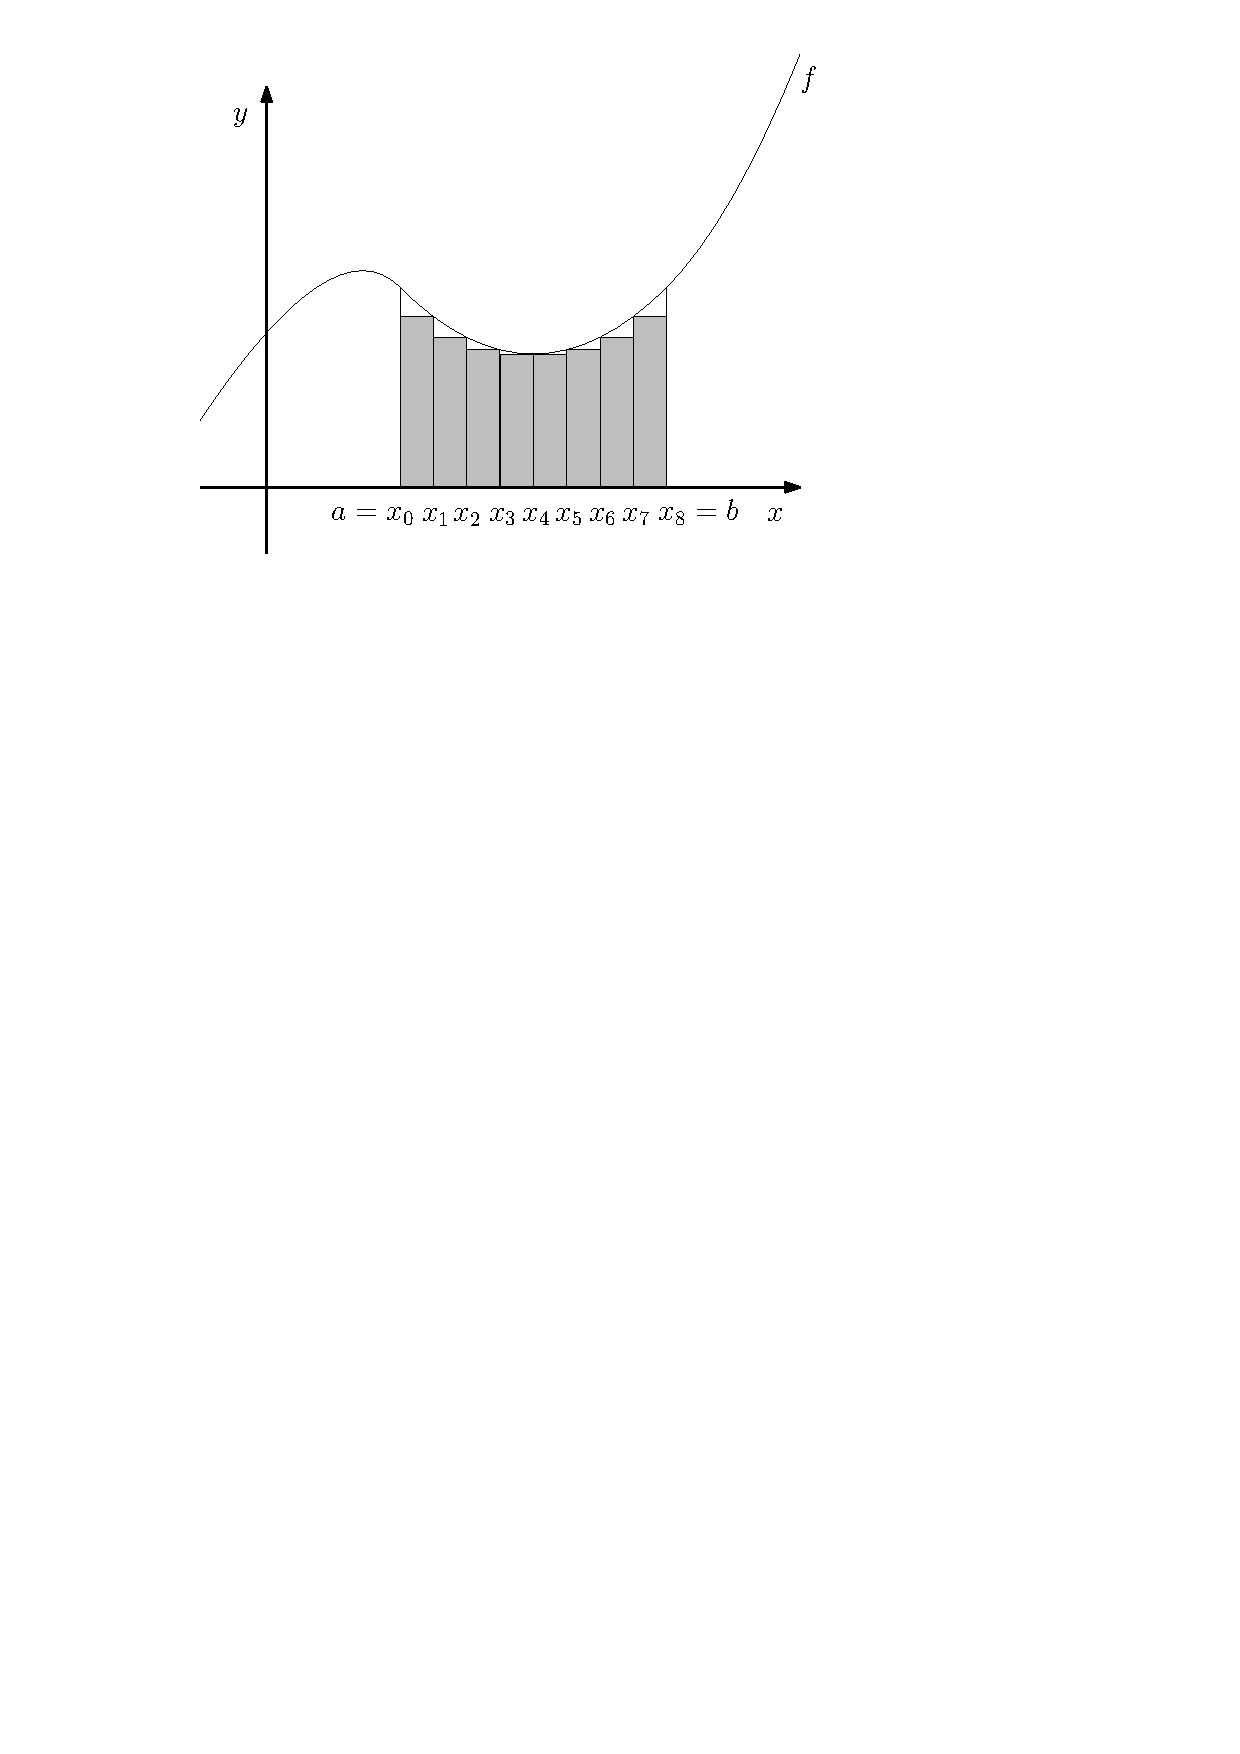
\includegraphics[scale=\normalipe]{ch01_urcity_integral_aproximace2.pdf}
	\caption{Aproximace plochy pod grafem funkce $f$ na intervalu $\langle a,b \rangle$ pomocí 8 obdélníků.}
	\label{fig:urcity_integral_aproximace2}
\end{figure}
Volbou stále "jemnějšího" dělení intervalu $\langle a,b \rangle$ se náš odhad bude zpřesňovat. Budeme-li mít tedy plochu aproximovanou $n$ obdélníky, pak\footnote{Symbolem $\approx$ značíme přibližnou rovnost (ve starších textech lze najít~i symbol $\doteq$).}
\begin{align}
\label{eq:aproximace_plochy_pod_grafem}
S \approx (x_1-x_0) \cdot \min\limits_{x_{0} \leq x \leq x_1}{f(x)} +\cdots + (x_n-x_{n-1}) \cdot \min\limits_{x_{n-1} \leq x \leq x_n}{f(x)}.
\end{align}
Pro rostoucí $n$, tedy počet dílčích intervalů $\langle x_{i-1},x_i \rangle$, se bude rozdíl $x_i-x_{i-1}$ blížit nule (obdélníky se budou "zužovat"). V konečném důsledku bude rozdíl $x_i-x_{i-1}$ "nekonečně malý"~a součet uvedený výše u aproximace v obrázku \ref{eq:aproximace_plochy_pod_grafem} přejde v integrál
\begin{align*}
S=\int_{a}^{b}{f(x)\,\dx},
\end{align*}
kde rozdíl $x_i-x_{i-1}$ přešel v diferenciál $\dx$~a minimum $\min\limits_{x_{n-1} \leq x \leq x_n}{f(x)}$ přešlo přímo ve funkční hodnotu $f(x)$.\par
V matematice značíme součty pomocí řeckého symbolu $\sum$ (velké písmeno \emph{sigma}). Proto se čtenář může často setkat v jiných textech se zápisem
\begin{align*}
S \approx \sum_{i=1}^{n}{(x_i-x_{i-1}) \cdot \min\limits_{x_{i-1} \leq x \leq x_i}{f(x)}}.
\end{align*}
Prohodíme-li činitele v součinu, pak už je o něco jednodušeji vidět přechod v integrál, který jsme popsali výše
\begin{align*}
\sum_{i=0}^{n}{\overbrace{\min\limits_{x_{i-1} \leq x \leq x_i}{f(x)}}^{\rightarrow f(x)} \cdot \underbrace{(x_i-x_{i-1})}_{\rightarrow \dx}} \longrightarrow \int_{a}^{b}{f(x)\,\dx}.
\end{align*}

Toto je velmi zjednodušené vysvětlení určitého integrálu,~avšak hlavní myšlenkou bylo právě ono potenciálně "nekonečné dělení", které bylo jedním z příkladů využití \textbf{nekonečně malých veličin}. (Zde konkrétně roli nekonečně malé veličiny zastávala postupně zmenšující se šířka obdélníků kvůli "zjemňování" dělení.)\par
Na podobných úvahách jsou založeny různé další pojmy v matematické analýze, jako např. \emph{limita}~nebo i \emph{derivace}. Je~však nutno si uvědomit, že co je nám známo dnes, nebylo zcela známo matematikům v 17. století. V této době se začal \emph{integrální}~a \emph{diferenciální} počet pořádně rozvíjet. Jejich tvůrci matematik \name{Gottfried~Wilhelm~Leibniz} (1646--1716)~a fyzik \name{Isaac~Newton} (1642--1726/27) základy své tehdejší úvahy o infinitezimálním počtu postavili právě na nekonečně malých veličinách. Problémem tehdy~však bylo, že tento pojem nebyl pořádně definován~a pravidla pro počítání s (aktuálně) nekonečně malými veličinami byla definována pouze velmi vágně. I přesto se~však integrální~a diferenciální počet ukázal být opravdu mocným nástrojem (hlavně ve fyzice). Postupně se~ale začaly nejasnosti v jejich samotných základech vyhrocovat, což nakonec vyústilo v období, které dnes nazýváme \emph{druhou krizí matematiky}\footnote{První krize matematiky nastala v dobách antického Řecka~a souvisela s objevem iracionálních čísel.}.\par
Problémy v matematické analýze se začaly odstraňovat až na počátku 19. století, kdy významnou roli sehrál ve dvacátých letech \name{Augustin~Louis~Cauchy} zavedením limity. Její formální definici~však podal později \name{Karl~Weierstrass}, která pracovala opět s potenciálním nekonečnem. (\cite{Fuchs2003}, str. 105--106.)